After geocoding, drought impacts are stored as tables with coordinates or region codes. These tables are hard to interpret on their own. An interactive map viewer was built to display the geocoded dataset in spatial form and support manual inspection before the validation analysis in the next section.

\subsection{Purpose}

The viewer was designed with three main aims.

The first aim is to check whether extracted impacts are credible. A user can inspect where impacts appear on the map, whether locations look reasonable for the Netherlands, and whether the extracted impact fields match the source news text. This combines spatial checking and text checking in one workflow.

The second aim is to study patterns across impact classes. The map can be restricted to one or more drought-impact categories (for example crop failure, groundwater depletion, or wildfire stress). Because each class keeps a fixed map colour, class-specific spatial patterns become easier to compare.

The third aim is to study patterns over time. Impacts are linked to article publication month, and the map can be limited to a selected period. This supports inspection of when certain impacts were reported, rather than only where they occurred.

\subsection{Point-Level Map}

\begin{figure}[htbp]
\centering
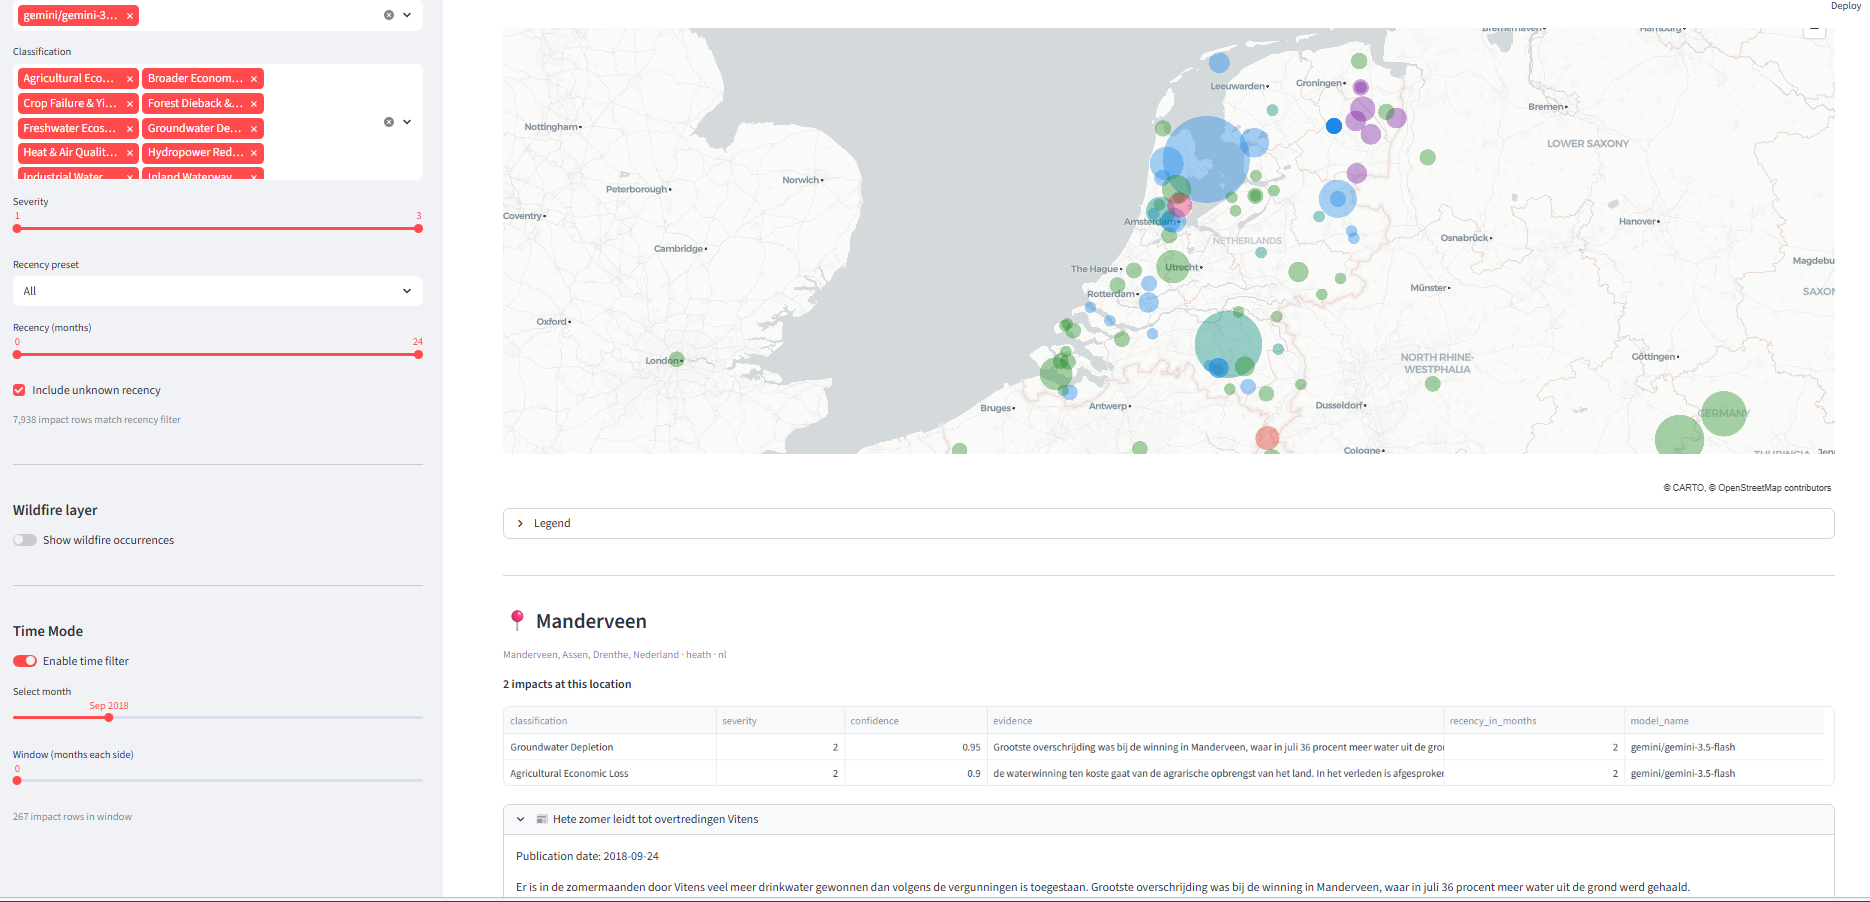
\includegraphics[width=0.97\textwidth]{figures/tool-overvieuw 2.png}
\caption{Point map and the news article view below.}
\label{fig:point-map}
\end{figure}

The point map displays geocoded impacts as markers on a Netherlands basemap (Figure~\ref{fig:point-map}). Impacts that share the same location mention are grouped into one marker. The number of impacts at a location controls marker size: places with more reported impacts appear as larger dots. Marker colour shows the dominant impact theme at that location. The original 20 impact classes are aggregated into six thematic groups: Agriculture (green), Water (blue), Fire and Heat (red-orange), Ecosystem (teal), Economy (purple), and Social (rose) (Table~\ref{tab:theme-colours}).

Marker transparency reflects the dominance of the leading impact theme. Locations where most impacts belong to a single theme appear more opaque, while locations with a more mixed impact profile appear fainter.

\begin{table}[htbp]
\centering
\caption{Thematic colour scheme used in the map viewer. The original 20 LLM impact labels are aggregated into six theme families.}
\label{tab:theme-colours}
\begin{tabular}{lll}
\toprule
Theme Family & Colour & Example Classes \\
\midrule
Agriculture & Green & Crop Failure, Irrigation Shortage, Agricultural Economic Loss \\
Water & Blue & Groundwater, Reservoir, Water Supply, Hydropower \\
Fire \& Heat & Red-orange & Wildfire Occurrence, Wildfire Risk, Heat \& Air Quality \\
Ecosystem & Teal & Freshwater Ecosystem, Forest Dieback, Wetland Loss \\
Economy & Purple & Broader Economic Disruption \\
Social & Rose & Social Impacts \\
\bottomrule
\end{tabular}
\end{table}



This view is suited to local inspection. It shows whether many impacts collapse onto the same place name, whether coordinates fall inside or outside the Netherlands, and whether geocoding appears too broad or too specific. Selecting a location opens a detail view with the impact records at that place and, when available, the related article text.

\subsection{Regional NUTS-3 Map}

\begin{figure}[htbp]
\centering
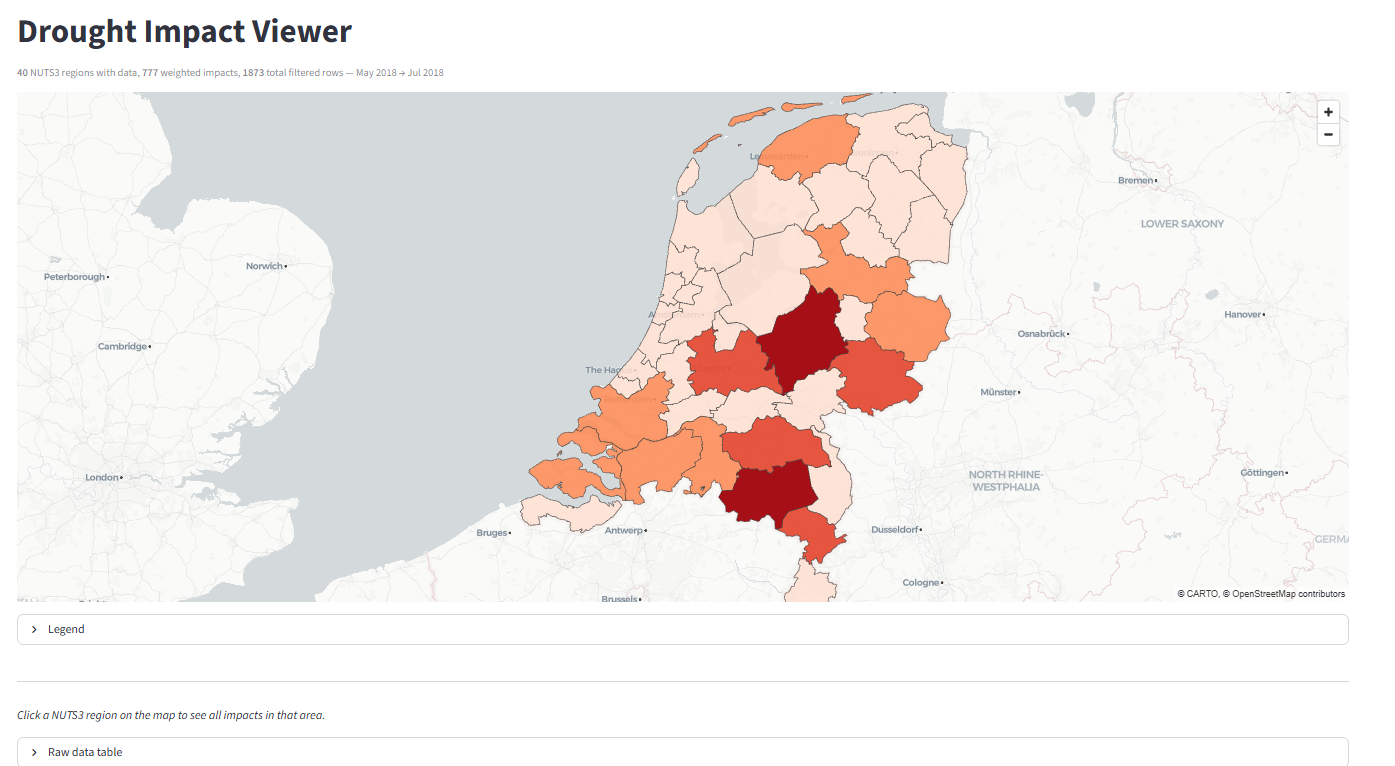
\includegraphics[width=0.8\textwidth]{figures/nuts-vieuw.png}
\caption{The NUTS-3 viewer with choropleth path colours}
\label{fig:nuts3-map}
\end{figure}

The regional map displays impacts on official NUTS-3 boundaries (Figure~\ref{fig:nuts3-map}). Impacts assigned to the same region are combined into one regional total. When a mention was split across multiple regions during geocoding, each part is counted through its \texttt{mention\_weight}, so broad phrases do not count as full impacts in every region.

Regional shading uses a colour scale from light to dark red. Regions with few or no impacts stay pale. Regions with more weighted impacts become darker. This makes regional concentration visible at a glance. Selecting a region shows the impacts assigned to that NUTS-3 unit and the linked article text where available.

The point map emphasises individual locations and local clustering. The regional map emphasises province-level structure and is better aligned with regional data used later in the thesis.

\subsection{Temporal and Class Views on the Map}

The same map can be filtered by impact class, severity, recency, and publication month. These filters change which markers or regions are drawn, not only which rows appear in a table. In practice, this allows class-specific maps for one drought category and month-specific maps for a chosen reporting window.

An optional wildfire layer can be added on top of either map. It shows observed fire occurrences from an external dataset and is included only as background context when inspecting drought-related fire reporting.

The next section uses these map views to assess geocoding quality and describe spatial and temporal patterns in the extracted impact dataset.




